\chapter{Redes Adversárias Geradoras}
\label{cha:gan}

%   ------------------------------------------------
%   ----- Redes Neurais como Modelos Geradores -----
%   ------------------------------------------------
\section{Redes Neurais como Modelos Geradores}
\label{sec:gan_nn_as_generative_model}



%   -----------------------------
%   ----- Redes Adversárias -----
%   -----------------------------
\section{Redes Adversárias}
\label{sec:gan_adversarial_nets}



%   ----------------------------
%   ----- Teoria dos Jogos -----
%   ----------------------------
\section{Teoria dos Jogos}
\label{sec:gan_game_theory}

Teoria dos Jogos é um enorme campo de estudos, geralmente mais comumente explorado pelos matemáticos, que tem um escopo bastante amplo e utiliza modelos matemáticos para oferecer visões importantes sobre cenários competitivos ou cooperativos que envolvam indivíduos que possam ter objetivos ou preferências diferentes \citep{myerson1997game}. Este campo de estudo tem uma ampla gama de aplicações em telecomunicações \citep{han2012game}, biologia \citep{smith1974theory}, economia \citep{Friedman1998, kreps1990game, gibbons1992game}, setor jurídico \citep{baird1998game}, administração \citep{sanfey2007social, camerer2011behavioral}, computação \citep{abraham2006distributed} etc.

RAND Corporation\footnote{O nome ``RAND'' vem de uma contração do termo, em inglês, ``research and development'' (\textbf{R}esearch \textbf{AN}d \textbf{D}evelopment).}, uma organização sem fins lucrativos independente, foi uma das instituições que mais estimulou o uso de cientistas e matemáticos para fins aplicados logo após a Segunda Guerra Mundial. Entre tantos outros matemáticos e cientistas brilhantes que participaram dos projetos da RAND estão John von Neumann, um pioneiro do computador digital moderno, e John Forbes Nash, que ganhou o Prêmio Nobel de Economia em 1994.

Segundo John von Neumann e Oskar Morgenstern:

\begin{formal}
\begin{quote}
\begin{flushright}
    \textcolor{citeblue}{\textquotedblleft \textit{The game is simply the totality of the rules which describe it.} \textquotedblright}\\ \citep{10.2307/j.ctt1r2gkx}
\end{flushright}
\end{quote}
\end{formal}

Ou seja, efetuando-se uma tradução livre, pode-se compreender que, segundo os professores Neumann e Morgenstern, o jogo é simplesmente a totalidade das regras que o descrevem.

Apesar do nome popularmente convidativo -- talvez por estar erroneamente associado a elementos meramente lúdicos -- não pode haver confusão quanto à importância dessa área, assim como o rigor dos modelos matemáticos envolvidos; tais confusões podem ocorrer devido à alta ambiguidade da linguagem coloquial \citep{10.2307/j.ctt1r2gkx}.

Na Subseção \ref{subsec:gan_prisoners_dilemma} será discutido mais sobre o \textbf{Dilema do Prisioneiro}, um exemplo de cenário que pode envolver cooperação e competição.




%   ----- Dilema dos Prisioneiro -----
\subsection{Dilema dos Prisioneiro}
\label{subsec:gan_prisoners_dilemma}

Originalmente, esse modelo havia sido proposto ao longo de 1950, na RAND, por Merrill Meeks Flood e Melvin Dresher; mais tarde, Albert William Tucker foi responsável por uma excelente interpretação do problema e pela atribuição do nome pelo qual é conhecido agora o modelo matemático, o \textbf{Dilema do Prisioneiro} \citep{poundstone1992prisoner}.

O cenário Dilema do Prisioneiro é composto por dois membros de uma gangue criminosa que são presos e mantidos separados um do outro e submetidos a um interrogatório, sem que haja qualquer tipo de comunicação entre eles durante todo esse processo. \textit{A priori}, o promotor tem provas suficientes para garantir a condenação de ambos os criminosos, mas apenas para crimes menores, o que não é suficiente para o promotor. Ambos os criminosos têm o direito de tomar a decisão de permanecer em silêncio ou de trair seu comparsa, delatando-o.

É importante enfatizar o fato de que, embora ambos os prisioneiros estejam cientes das possíveis consequências de cada situação, não se sabe sobre o que o outro decidiu fazer. Se o Prisioneiro A escolher cooperar com o Prisioneiro B, dependendo da estratégia adotada pelo Prisioneiro B, as consequências podem ser de 1 ano de prisão tanto para A quanto para B se o Prisioneiro B também cooperar com A; ou, se B denunciar A, 4 anos de prisão para A e imediata liberdade para B. Ao inverter as estratégias entre A e B, as penas são as mesmas, mudando apenas os presos. Porém, se ambos os presos escolherem denunciar seu parceiro, ambos serão sentenciados a três anos de prisão.

A Figura \ref{fig:prisoners_dilemma} contém um exemplo hipotético para o Dilema do Prisioneiro.

\begin{figure}[H]
    \centering
    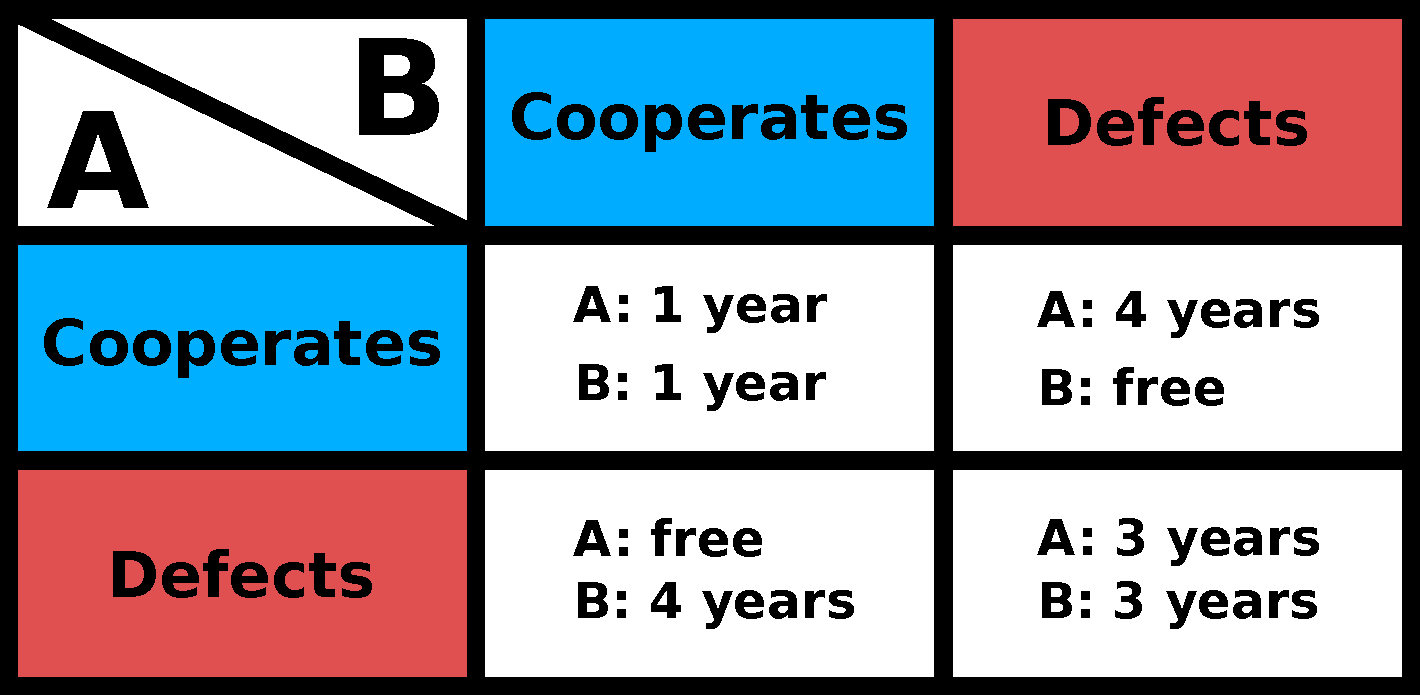
\includegraphics[width=0.60\textwidth]{figs/prisoners_dilemma_3.pdf}
    \caption{Estratégias e suas respectivas consequências para os prisioneiros A e B. A estratégia de cooperação significa que o prisioneiro ficará calado e aceitará as consequências; e a estratégia de desertar é trair seu parceiro denunciando-o pelo crime mais pesado.}
    \label{fig:prisoners_dilemma}
\end{figure}

O clássico Dilema do Prisioneiro, apresentado até agora, considera apenas uma ocorrência para ambos os prisioneiros envolvidos, mas não é suficiente para modelar adequadamente todas as situações possíveis; um algoritmo ainda mais flexível consideraria iterações \citep{press2012iterated}.

A Subseção \ref{subsec:gan_minmax} tratá uma regra de decisão muito interessante que pode ajudar a escolher a estratégia que melhor se adapte a ambos os prisioneiros.




%   ----- MinMax -----
\subsection{MiniMax}
\label{subsec:gan_minmax}

Esta subseção começa explicando alguns passos para se chegar à melhor decisão para o Dilema do Prisioneiro, seguindo o exemplo dado pela Figura \ref{fig:prisoners_dilemma}.

Numa primeira tentativa ingênua, um prisioneiro pode pensar em ficar quieto, cooperando com seu cúmplice, mas como não é possível saber qual será a estratégia de seu cúmplice, este prisioneiro corre o risco de ser condenado a 4 anos de prisão. Isto é, uma simples mudança de estratégia egoísta por parte do outro preso, sobre o qual não há controle, pode causar uma grande alteração no resultado da penalidade do primeiro preso, indo do mínimo (1 ano) para o máximo (4 anos). Esta é, então, uma estratégia muito arriscada. Por outro lado, o prisioneiro pode escolher denunciar seu companheiro; isso certamente garantiria ao outro preso uma sentença mínima de 3 anos e um máximo de 4 anos, além de colocar o prisioneiro que tomou tal decisão em posição de poder sair em liberdade, desde que seu parceiro também não o entregue.

Para evitar as piores consequências possíveis para ambos os criminosos, eles têm que alcançar um forte \textit{equilíbrio de Nash} \citep{Nash48}, ou seja, chegar a uma posição cujo resultado para um deles não receberia uma melhoria significativa se mudasse sua estratégia unilateralmente. A ideia aqui, portanto, seria minimizar a sentença máxima; esta é uma regra de decisão chamada \textit{MiniMax}\footnote{É possível encontrar variações deste termo, tais como \textit{MinMax}, ou \textit{Max Min}, ou MM, dependendo da referência utilizada.} \citep{v.Neumann1928, blackwell1956analog, willem1997minimax}.

Assim, continuando com o exemplo exposto na Figura \ref{fig:prisoners_dilemma}, o movimento mais seguro para ambos seria optar por delatar seu cúmplice, pois quem delatar terá sua pena superiormente limitada a 3 anos; Além disso, se o seu companheiro não fizer o mesmo, em vez de ser condenado à prisão, será libertado.



%   ---------------
%   ----- GAN -----
%   ---------------
\section{Redes Adversárias Geradoras}
\label{sec:gan_gan}

Explorando conceitos de Teoria dos Jogos e de Aprendizagem Profunda, foi possível formular um novo tipo de abordagem, utilizando duas redes neurais como jogadores adversários de um jogo competitivo; assim, foram propostas as Redes Adversárias Geradoras (\textbf{GAN}, do inglês \textit{Generative Adversarial Networks}) \citep{NIPS2014_5423}.

Neste jogo competitivo para dois jogadores, existe um conjunto de dados já bem preparado, composto por amostras do mesmo tipo, escolhidas de forma adequada, mas com valores de atributos diferentes. O primeiro jogador, $D$, tem o objetivo de discriminar se uma amostra veio do conjunto de dados original ou não; o segundo, $G$, deve capturar a distribuição do conjunto de dados original e usá-la para gerar amostras completamente novas. Assim, enquanto um dos jogadores pretende gerar a imitação perfeita dos dados originais, o outro jogador tenta ser o melhor identificador de falsificações possível.

Como foi dito neste capítulo, ambos os jogadores deste jogo são redes neurais artificiais e, como há uma dependência de treinamento, este passo deve ocorrer gradualmente e concomitantemente para ambos os jogadores, caso contrário, dado que os jogadores estão jogando um contra o outro, caso contrário, pode ocorrer um desequilíbrio de evolução em favor de um dos atores, que tenderá a tornar o processo evolutivo cada vez mais desfavorável para um lado e, assim, em vez de conseguir uma boa evolução para ambos, apenas um deles evoluirá minimamente se comparado ao outro, o que sequer garante que o processo terá sido bom para ao menos um dos jogadores.

O modelo matemático baseado na regra de decisão Minimax, da Subseção (\ref{subsec:gan_minmax}), que é utilizado pelo algoritmo da GAN, pode ser visto na Equação (\ref{eq:minimax}).

\begin{equation}
    \min_{G} \max_{D} V\left(D, G\right) = \mathbb{E}_{\pmb{x}\thicksim p_{\text{data}}\left(\pmb{x}\right)}\left[\log D\left(\pmb{x}\right)\right] + \mathbb{E}_{z\thicksim p_{z}\left(z\right)}\left[\log \left(1 - D\left(G\left(z\right)\right)\right)\right],
    \label{eq:minimax}
\end{equation}

onde $V$ é a função de valor; $D$ é o Discriminador, um perceptron multi-camada que gera a probabilidade de $\pmb{x}$ ter sido originado dos dados legítimos em vez da distribuição $p_{G}$; $G$ é o Gerador (jogador); $p_{\text{data}}$ é a distribuição de dados; e $p_{\text{\pmb{z}}}$ é uma \textit{a priori} nas variáveis de ruído de entrada.

O treinamento de Redes Adversariais Generativas usa um método baseado em Gradiente Descendente Estocástico, que pode ser visto no Algoritmo \ref{alg:gan_train} \citep{NIPS2014_5423}.


\begin{algorithm}
\caption{Treinamento de Redes Adversárias Geradoras com Gradiente Descendente Estocástico por mini-lotes. O número de etapas a serem aplicadas ao Discriminador, $k$, é um hiper-parâmetro \citep{NIPS2014_5423}.}
\label{alg:gan_train}
\begin{algorithmic}[1]

\For {número de iterações de treinamento}
    \For {$k$ passos}
        \parState {$\sbullet[1.5]$ Amostrar lote de $m$ amostras ruidosas $\set[\big]{\pmb{z}^{\left(1\right)}, \dots, \pmb{z}^{\left(m\right)}}$ de ruído \textit{a priori} $p_{g}\left(\pmb{z}\right)$.}
        
        \parState {$\sbullet[1.5]$ Amostrar lote de $m$ exemplos $\set[\big]{\pmb{x}^{\left(1\right)}, \dots, \pmb{x}^{\left(m\right)}}$ da distribuição geradora de dados $p_{\text{data}}\left(\pmb{x}\right)$.}
        
        \parState {$\sbullet[1.5]$ Atualiza o discriminante aumentando seu gradiente estocástico:
        \begin{equation*}
            \nabla_{\theta_{d}} \dfrac{1}{m} \sum_{\mathclap{i=1}}^{m} \left[\log D\left(\pmb{x}^{\left(i\right)}\right) + \log \left(1-D\left(G\left(\pmb{z}^{\left(i\right)}\right)\right)\right)\right].
        \end{equation*}}
    \EndFor
    
    \parState {$\sbullet[1.5]$ Amostra lote de $m$ amostras ruidosas $\set[\big]{\pmb{z}^{\left(1\right)}, \dots, \pmb{z}^{\left(m\right)}}$ de ruído \textit{a priori} $p_{g}\left(\pmb{z}\right)$.}
    
    \parState {$\sbullet[1.5]$ Atualiza o gerador diminuindo seu gradiente estocástico:
    \begin{equation*}
        \nabla_{\theta_{d}} \dfrac{1}{m} \sum_{\mathclap{i=1}}^{m} \log \left(1-D\left(G\left(\pmb{z}^{\left(i\right)}\right)\right)\right).
    \end{equation*}}
\EndFor

\noindent As atualizações baseadas em gradiente podem utilizar qualquer regra de aprendizagem padrão baseada em gradiente.

\noindent Este algoritmo utilizou $k = 1$ e o utilizou momento como regra de aprendizagem padrão.

\end{algorithmic}
\end{algorithm}




%   --------------------------------
%   ----- Aplicação em Imagens -----
%   --------------------------------
\section{Aplicação em Imagens}
\label{sec:gan_applications_to_images}

